\section{LHC Phase 2 Secondary Collimator Jaw Material}

The phase 2 secondary collimators are proposed as an addition to the current phase 1 secondary collimators. They have stringent mechanical requirements, particularly due to the neccessity to withstand impacts by a limited number of bunches in the LHC during injection. In addition they must meet a stringent limit on beam impedance - new devices in the LHC must not increase the total impedance of the machine due to the stability limits imposed due to the existing large transverse and longitudinal impedance. If possible, the effective impedance in the machine should be reduced during operation. The requirements for the material requirements are detailed and summarised in [cite a. dallocchio phase 2 advanced materials].

To meet the strict requirements of the differing physical requirments on the jaw material, both from a mechanical point view and an impedance point of view a number of different jaw design solutions have been proposed. These include both single jaw material designs, mixtures of composites and pure metals, and varities on a design including ceramic. The proposed jaw material combinations are listed below:

\begin{enumerate}
\item{GlidCop, a copper compositie including aluminium oxide particles[ref]. The conductivity is marginally worse than pure copper (see Tab.~\ref{tab:phase2-cond}), but the addition of the aluminium oxide greatly increases the resistance to thermal softening and increases the strength at high temperatures.}
\item{Molybdenum - An metal with good mechanical properties and a conductivity comparable to copper.}
\item{Copper Diamond Composite - A copper composite formed by hot pressing copper with the addition of boron powder and small synthetic diamonds. Produces a very mechanically robust material.}
\item{Molybdenum Diamond Composite - As with the above, a molybdenum compositie formed by the use of sintering molybdenum with artificial diamonds.}
\item{Carbon reinforced carbon (CFC) - The current material of the phase 1 secondary collimators. Included for comparison.}
\end{enumerate}

More information on the material choices can be found in [cite AD/AB papers]. The conductivities of the different materials can be found in Tab.~\ref{tab:phase2-cond}. The layouts of the various possible jaw designs can be found in Fig.~\ref{fig:phase2-jaw-designs}.

\begin{table}
\caption{The electrical conductivity of the different jaw materials proposed for use in the phase 2 design. All results are given for measurements at room temperature (20$^{o}$C)}
\begin{center}
\begin{tabular}{c | c }
Chapter & Completeness \\ \hline
Glidcop & $5.4 \times 10^{7}$ \\ \hline
Molybdenum & $1.87 \times 10^{7}$ \\ \hline
Copper Diamond Compositie (CuCD) & $1.25 \times 10^{7}$ \\ \hline
Molybdenum Diamond Composite (MoCD) & $5.5 \times 10^{6}$ \\ \hline
Graphite & $7 \times 10^{4}$ \\ \hline
\end{tabular}
\end{center}
\label{tab:phase2-cond}
\end{table}

\begin{figure}
\subfigure[]{
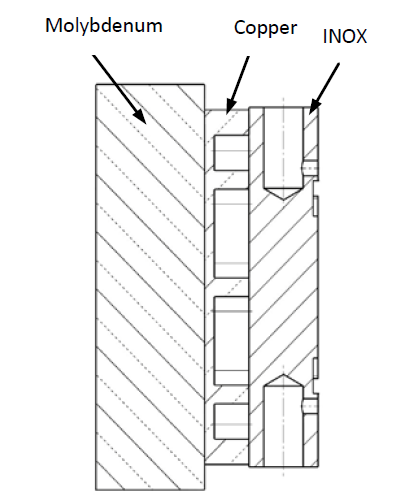
\includegraphics[width=0.45\textwidth]{LHC_Collimation_Upgrades/figures/mo-geo.png}
\label{fig:phase-2-moly}
}
\subfigure[]{
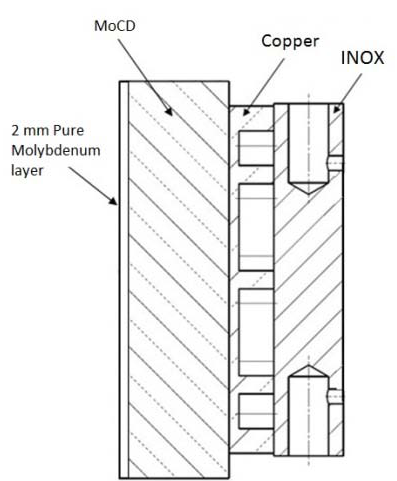
\includegraphics[width=0.45\textwidth]{LHC_Collimation_Upgrades/figures/mo-mocd-geo.png}
\label{fig:phase-2-molycd}
}
\label{fig:phase-2-jaw-designs}
\caption{A number of the proposed jaw designs for the phase 2 secondary collimators. \ref{fig:phase-2-moly} shows the jaw made entirely from molybdenum. Glidcop maybe substituted for molybdenum in this design. \ref{fig:phase-2-molycd} shows the jaw made from a mixture of molybdenum diamond composite with a 2mm coating of molybdenum on the surface. The composite ensure a mechanically strong jaw, whilst the coating screens the higher resistivity composite and provides a smooth surface on the beam-facing part of the jaw. In this case the composite maybe substituted with copper diamond composite, and likewise the coating may be replaced with GlidCop.}
\end{figure}

\subsection{Impedance Studies and Analysis}

To analyse the jaw material impedance the Mounet model [ref N. Mounet thesis/notes] for parallel plates with infinite layers is used. This model assumes infinite parallel plates with n-layers of material. It supports non-symmetric structures in addition. The representation of this structure is shown in Fig.~\ref{fig:mounet-model}. For this model we assume a jaw seperation of 4mm (half-width of 2mm), the closest nominal seperation of the secondary collimators.

The frequency range of concern is determined by the instability mechanism driving the stability limit in the LHC. It has been demonstrated that this range of concern is from 11.8kHz up to some number of GHz[cite phase 2 conf note] in the transverse plane, driven by loss due to tune spread over an optical resonance. This neccessitates investigating the transverse beam coupling impedance over a very large frequency range, hence the choice of using an analytical method of investigation.

\begin{figure}
\label{fig:mounet-model}
\caption{The physical model of the Mounet model of parallel plate impedance. Note that the two sides of the structure do not have to be symmetric. The materials maybe any material provided it's frequency dependent properties are well defined.}
\end{figure}

\begin{figure}
\subfigure[]{
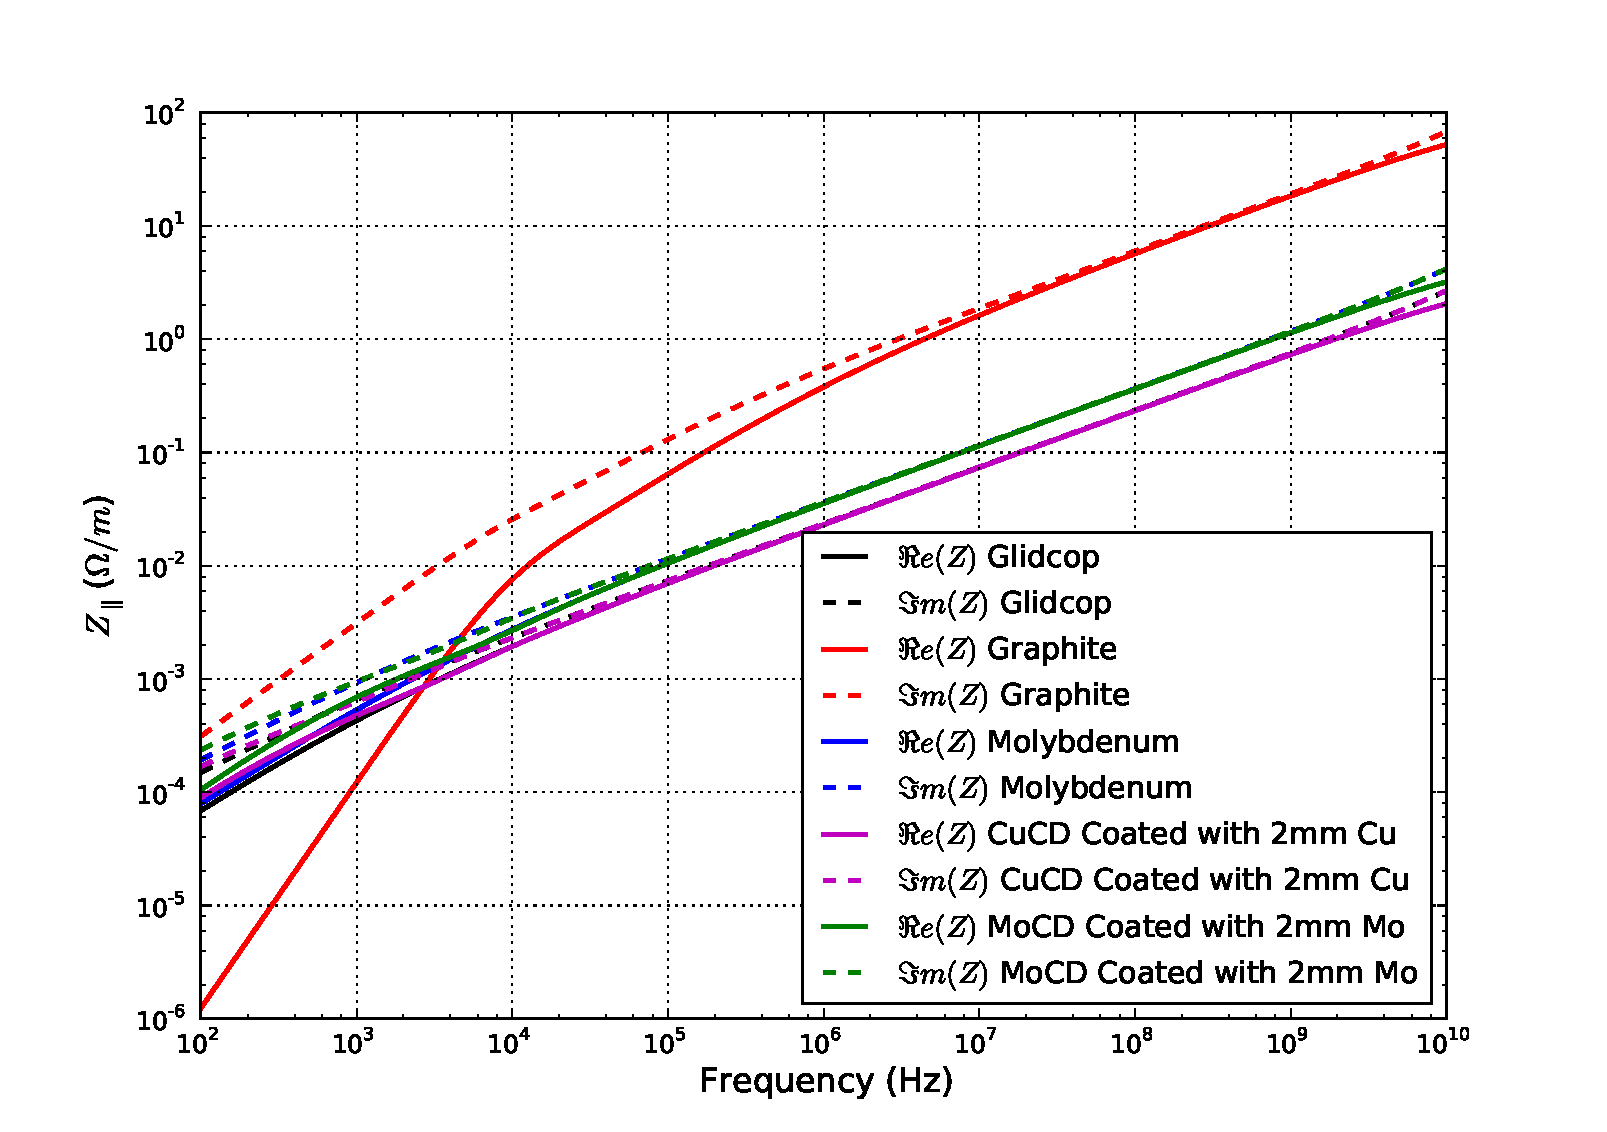
\includegraphics[width=0.5\textwidth]{LHC_Collimation_Upgrades/figures/longitudinal.pdf}
\label{fig:phase-2-long}
}
\subfigure[]{
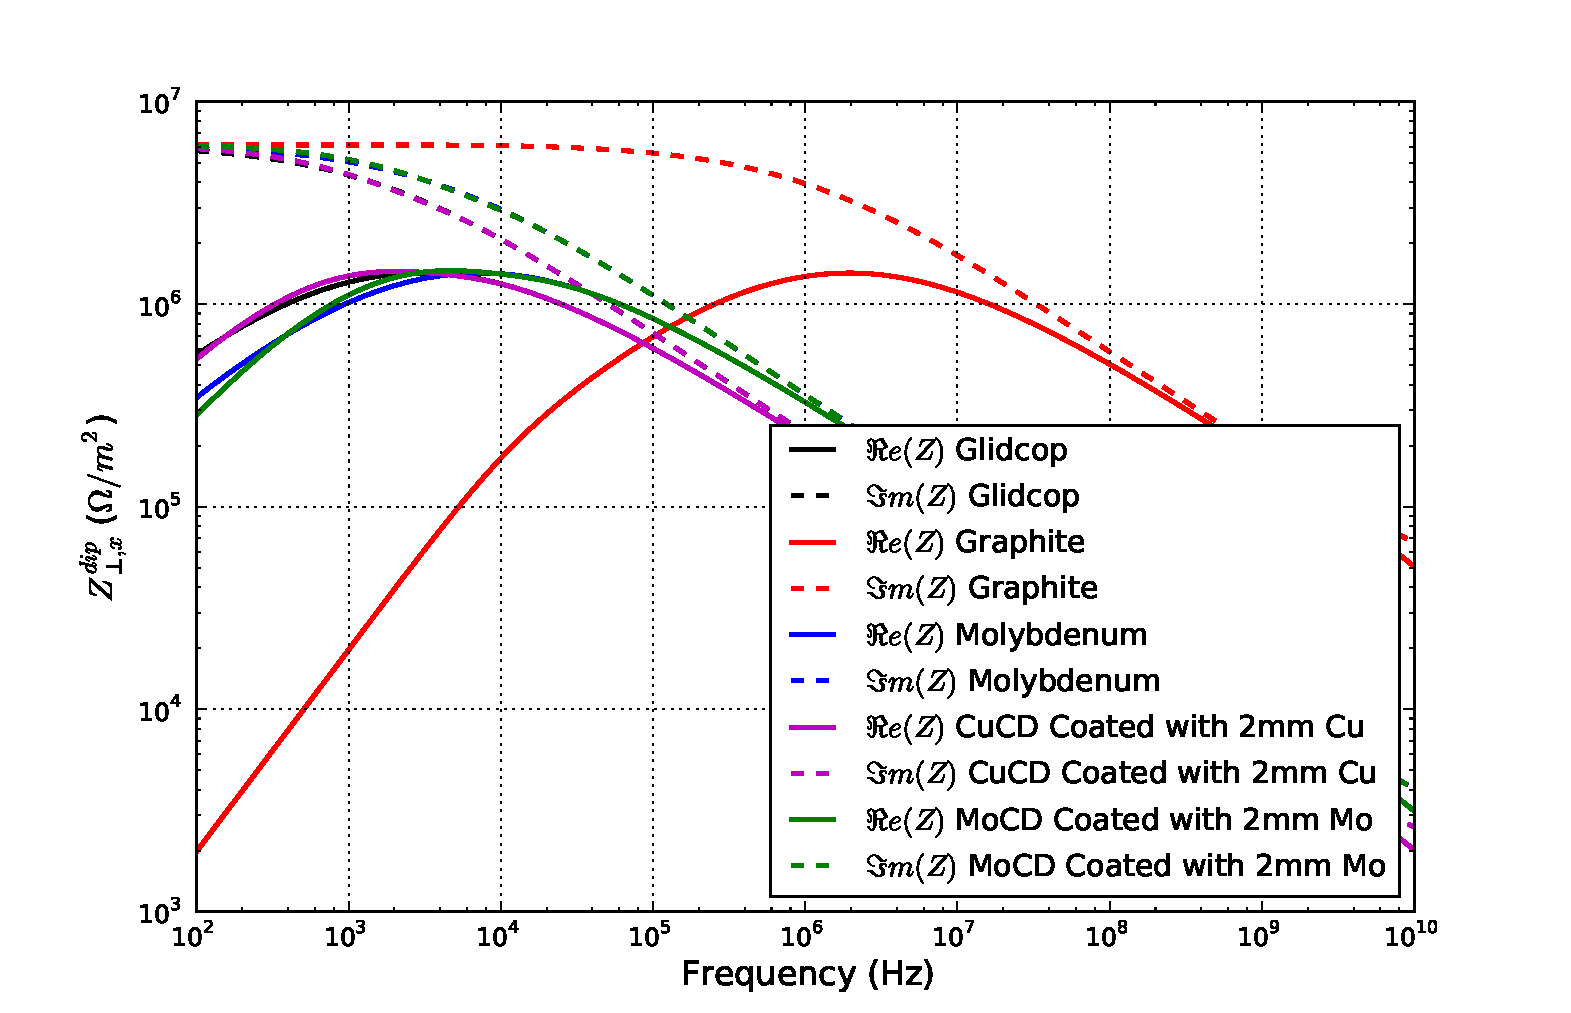
\includegraphics[width=0.5\textwidth]{LHC_Collimation_Upgrades/figures/horizDipolar.pdf}
\label{fig:phase-2-horzdip}
}
\subfigure[]{
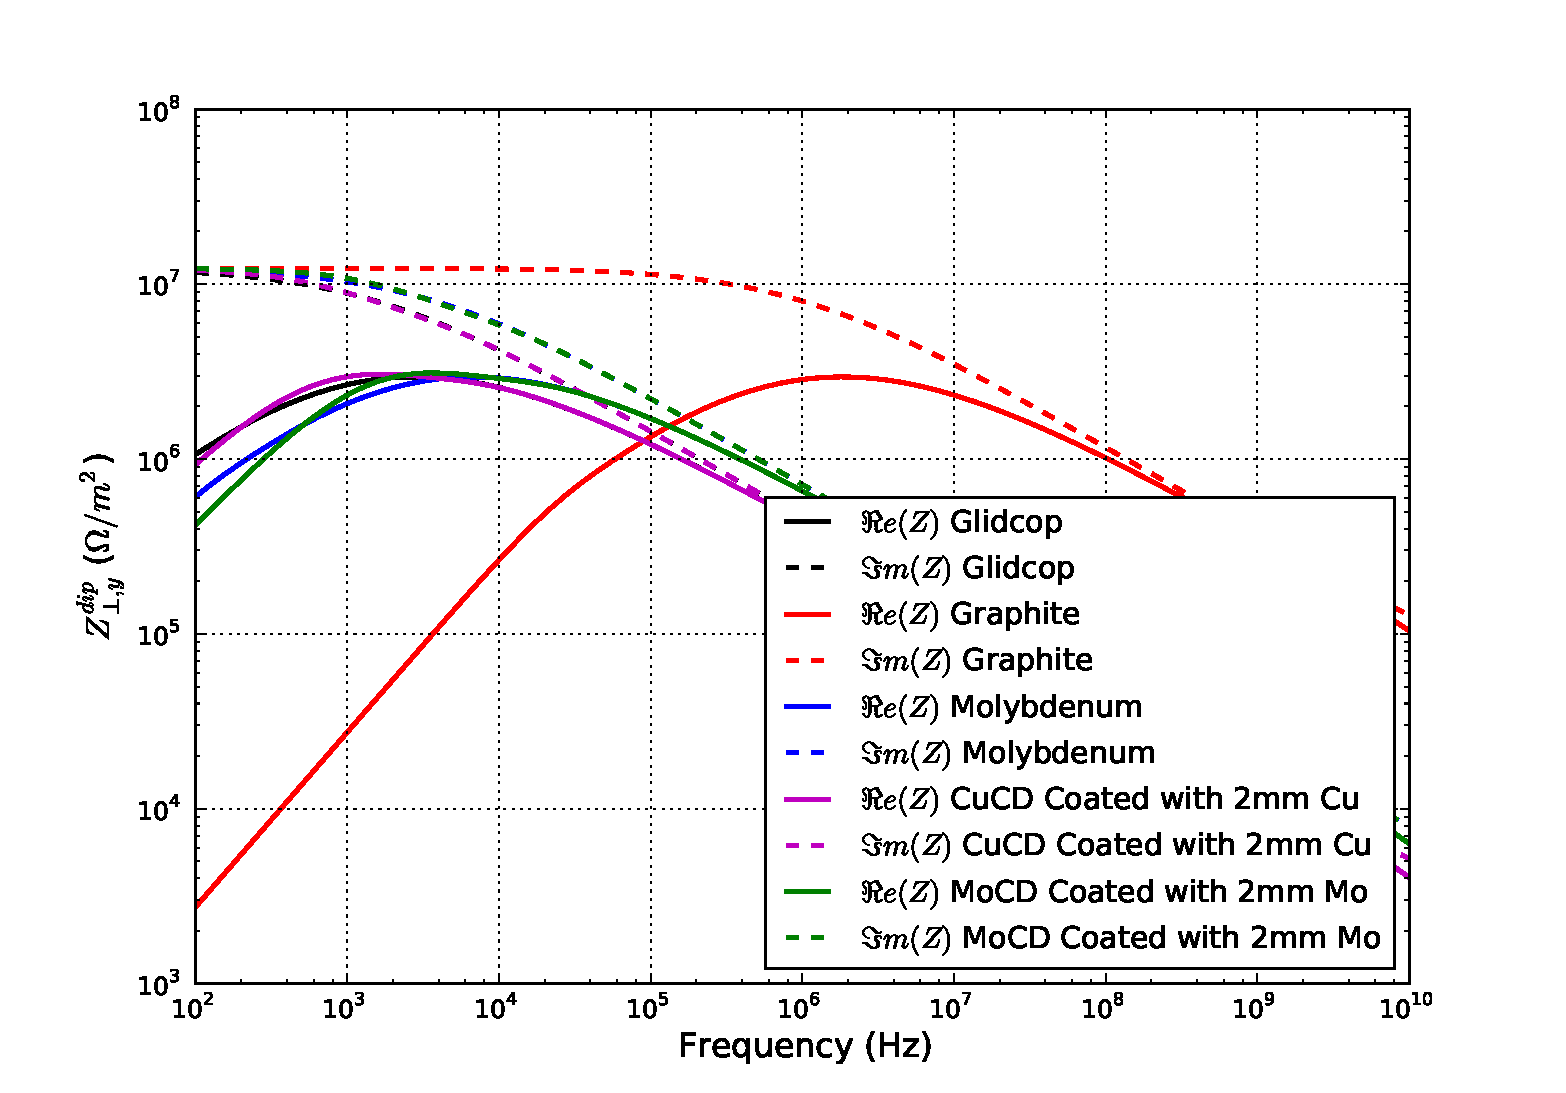
\includegraphics[width=0.5\textwidth]{LHC_Collimation_Upgrades/figures/vertDipolar.pdf}
\label{fig:phase-2-vertdip}
}
\subfigure[]{
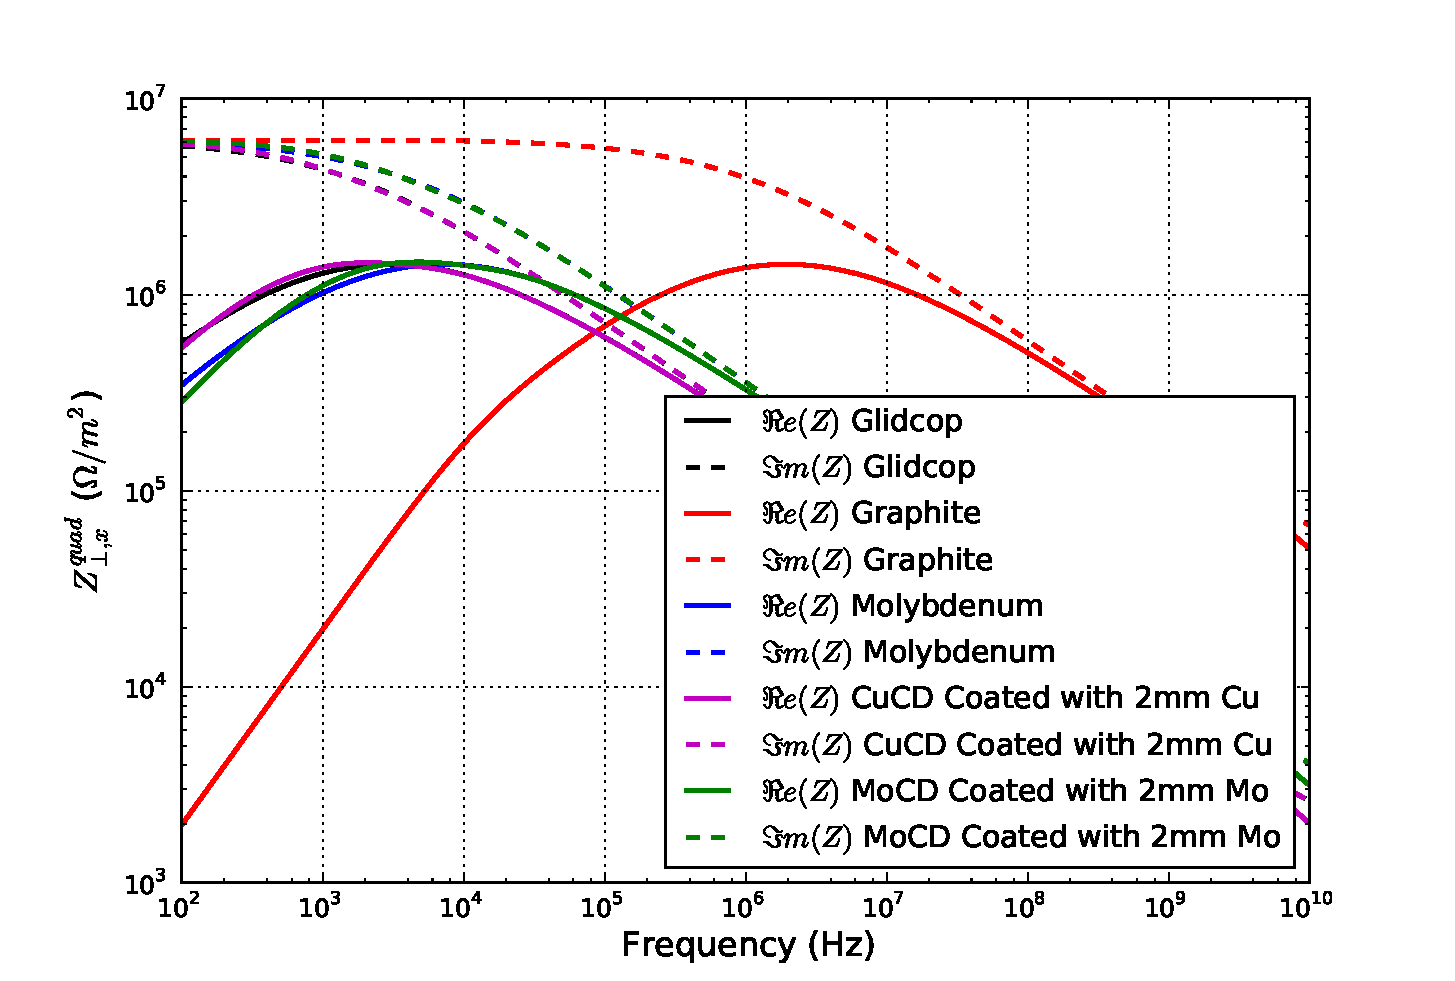
\includegraphics[width=0.5\textwidth]{LHC_Collimation_Upgrades/figures/horizQuadrupolar.pdf}
\label{fig:phase-2-horzquad}
}
\subfigure[]{
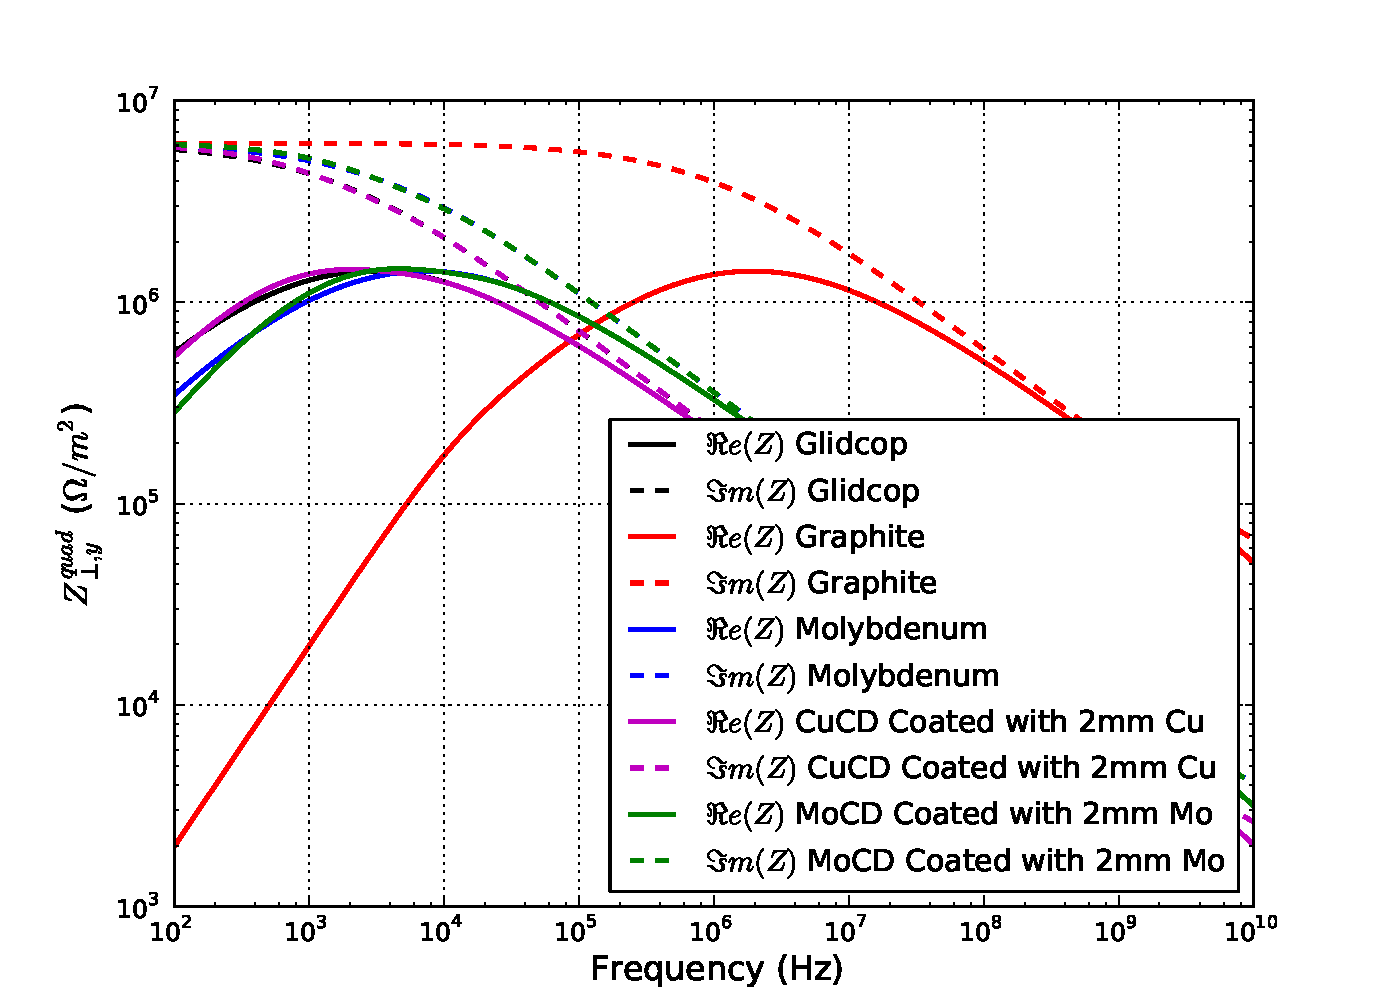
\includegraphics[width=0.45\textwidth]{LHC_Collimation_Upgrades/figures/vertQuadrupolar.pdf}
\label{fig:phase-2-vertquad}
}
\label{fig:phase-2-jaw-impedances}
\caption{The impedances of different jaw materials for the phase 2 secondary collimators. \ref{fig:phase-2-long} The longitudina impedance, \ref{fig:phase-2-horzdip} the horizontal dipolar impedance, \ref{fig:phase-2-vertdip}, the vertical dipolar impedance, \ref{fig:phase-2-horzquad} the horizontal quadrupolar impedance and \ref{fig:phase-2-vertquad} the vertical quadrupolar impedance.}
\end{figure}

The beam coupling impedances for the various jaw materials is shown in Fig.~\ref{fig:phase-2-jaw-impedances}. From the consideration of the longitudinal impedance, the collimator jaw material is not a significant contirbutor to the machine impedance. The significant concern is the transverse impedance. It can be seen from \cref{fig:phase-2-horzdip, fig:phase-2-vertdip, fig:phase-2-horzquad, fig:phase-2-vertquad} that all the potential jaw materials reduce the imaginary component of the transverse impedance (dipolar and quadrupolar) above $10^{3}$ Hz. By comparison to the change in tune shift discussed in Sec.~\ref{sec:tune-shift-bunch-int} it can be seen that this reduces the magnitude of the imaginary component of the tune shift - i.e. the change in betatron tune is reduced. 

Conversely, the peak of the real component of the transverse impedance is moved to lower frequencies as the conductivity of the innermost jaw material increases (shown in greater magnitude for the vertical dipolar impedance in Fig.~\ref{fig:phase-2-vertdip-zoom}). Importantly, this causes the high conductivity jaw materials to present a larger real component of the impedance in the important frequency range from $10^{4}-10^{5}$ Hz. Reviewing Sec.~\ref{sec:growth-time-chrom} it can be seen that this produces an decrease in the growth time. 

\begin{figure}
\begin{center}
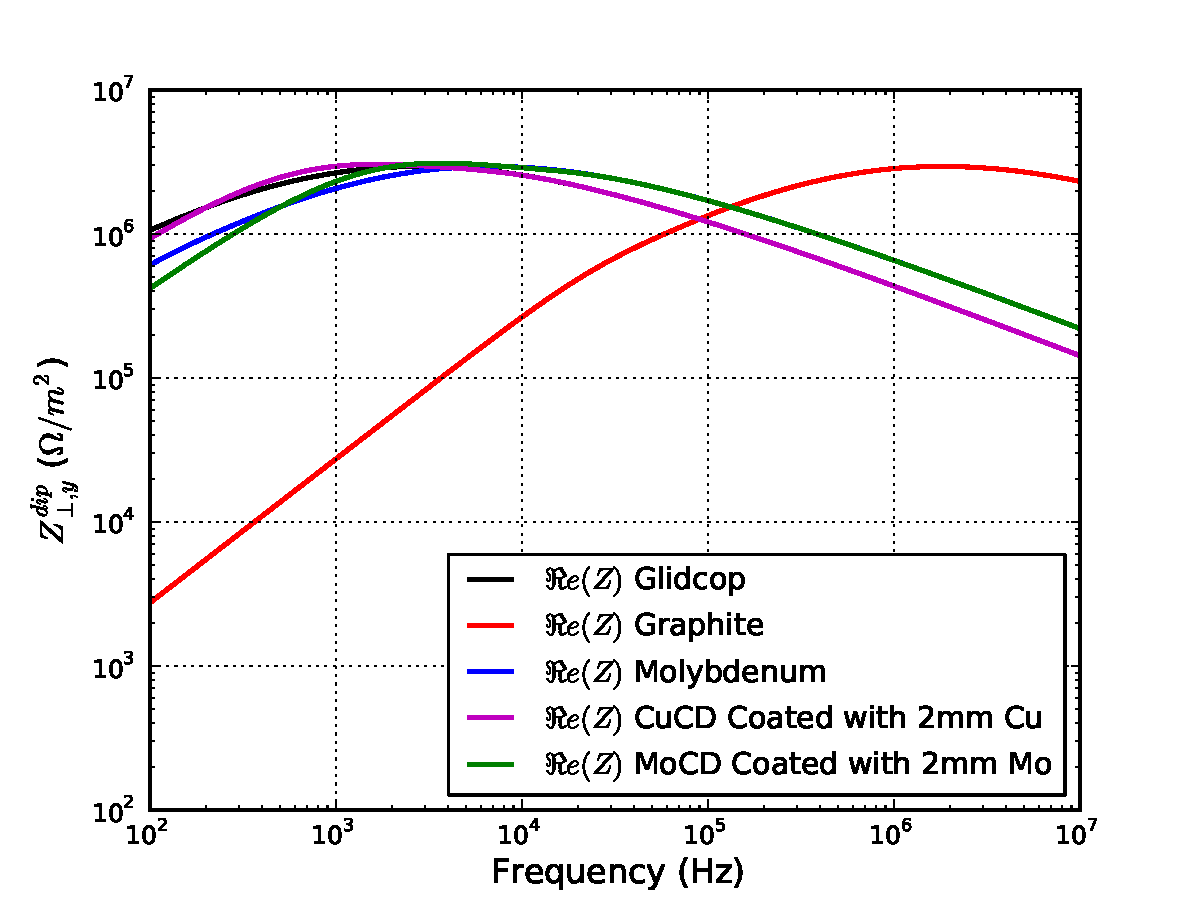
\includegraphics[width=0.7\textwidth]{LHC_Collimation_Upgrades/figures/vertDipolarZoom.pdf}
\end{center}
\label{fig:phase-2-vertdip-zoom}
\caption{The real component of the vertical dipolar impedance of the various collimator jaw materials assuming a 2mm half gap.}
\end{figure}
